% !TEX root = main.tex

\chapter{Experimental system and techniques}
In this chapter, the essential parts of the already existing setup on top of which the addressing system has been built are described. Calcium-40 ions are used in the experiment and the implementation of several techniques for trapping and manipulating these ions are discussed. Furthermore, the addressing setup utilizes 393 nm light and the laser emitting this light was already installed by H. Hainzer\footnote{In Helene's master project, the 393 nm laser (MSquared Ti:Sa) and the ion cavity were locked to an ultrastable reference cavity. The linewidth of the MSquared Ti:Sa laser was measured to be <100 Hz with a drift rate of 202(1) mHz/s} \cite{helene}, thus that setup is briefly presented. Finally, the experiment can be controlled remotely via computers, an overview of how it is implemented is also given.

\section{Ion trap and key techniques}
\subsection{Calcium Ions}
\label{sec:calciumion}
% \begin{figure}
% \centering
% 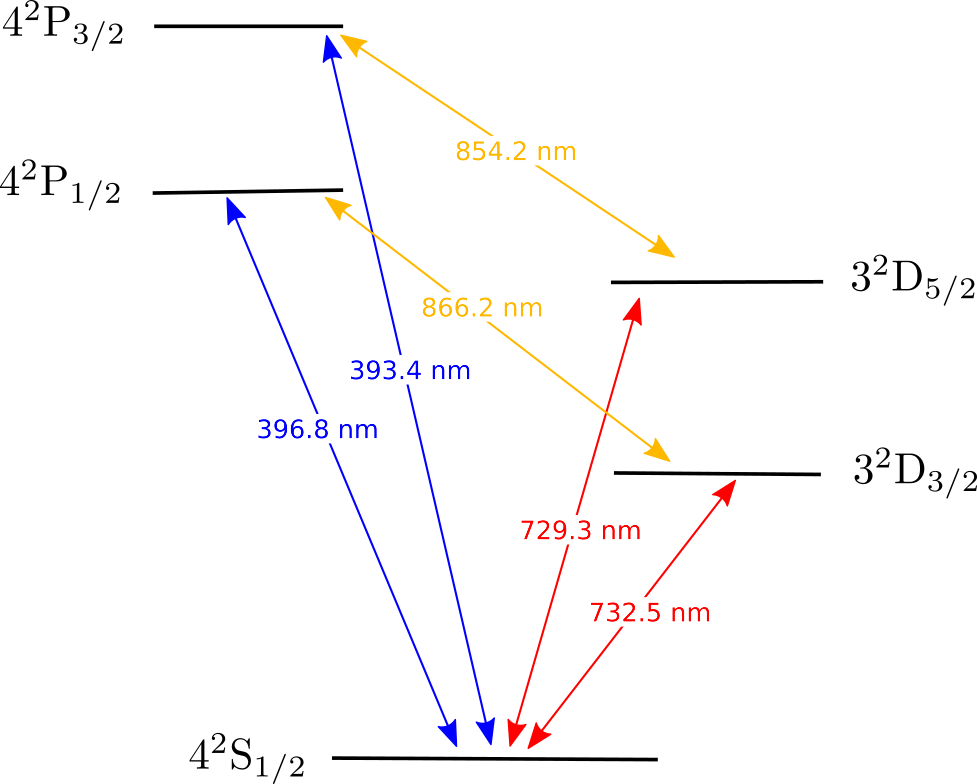
\includegraphics[width = .6 \textwidth]{calciumscheme}
% \caption{}
% \label{calciumscheme}
% \end{figure}
Ions with a single valence electron are attractive given their simple level schemes and straightforward cooling schemes, examples include beryllium \cite{beryllium}, barium \cite{barium}, strontium \cite{strontium}, calcium \cite{calcium}, ytterbium \cite{PhysRevA.44.R20}, and magnesium \cite{magnesium}. In our experiment we trap $^{40}\text{Ca}^+$, the most abundant isotope of calcium. In Figure \ref{qubitschemereference} the level scheme of the valence electron is presented. There is no hyperfine structure as $^{40}\text{Ca}^+$ does not posses a nuclear spin. Two short lived excited states $\text{P}_{1/2}$, and $\text{P}_{3/2}$ ($1/\Gamma \sim 7.7$ ns, and $1/\Gamma \sim 7.4$ ns, respectively) are connected to S via dipole transitions. Due to the short lifetimes of these two states, they are suitable for laser cooling and state detection.
 The states $\text{D}_{3/2}$ and $\text{D}_{5/2}$ are metastable ($ 1/\Gamma \sim 1$ s) and are coupled to the S state via electric quadrupole transitions. An optical qubit can be implemented in the states $\text{S}_{1/2}$ and $\text{D}_{5/2}$, as the lifetime of the $\text{D}_{5/2}$ state is longer than typical operation times \cite{calciumqubit}. Other choices for qubit implementations have been explored, for instance in the Zeeman levels of the $\text{S}_{1/2}$ manifold \cite{Ruster2016}. Table \ref{transitiontable} summarizes details about the different transitions, and what they are used for. A more detailed description and implementation is discussed in the next section.

\begin{table}[H]
\centering
\begin{tabular}{c c c c c c}
 \toprule
    {Transition} & { $\lambda$ (nm)} & {Decay rate $\Gamma$} & Lifetime $\tau$ & BR & {Main use here} \\ \midrule
   $\text{S}_{1/2} \leftrightarrow \text{P}_{1/2}$ & 396.847 & $2\pi \times 20.8$ MHz & 7.7 ns & 94\% &Cooling and imaging \\
    $\text{S}_{1/2} \leftrightarrow \text{P}_{3/2}$  & 393.366 & $2\pi \times 21.4$ MHz & 7.4 ns & 94\% &Photon generation\\ \midrule
   $\text{S}_{1/2} \leftrightarrow \text{D}_{3/2}$ & 732.389 & $2\pi \times 0.132$ Hz & 1.080 s & - & - \\
    $\text{S}_{1/2} \leftrightarrow \text{D}_{5/2}$  & 729.147 & $2\pi \times 0.136$ Hz & 1.045 s & - & Manipulate optical qubit \\\midrule
    $\text{P}_{1/2} \leftrightarrow \text{D}_{3/2}$  & 866.214 &  $2\pi \times 1.70$ MHz  &  94.3 ns & 6\% & Repumping \\
    $\text{P}_{3/2} \leftrightarrow \text{D}_{5/2}$  & 854.209 & $2\pi \times 1.34$ MHz & 101 ns & 5.3\%  & Cavity photon  \\
    $\text{P}_{3/2} \leftrightarrow \text{D}_{3/2}$  & 849.802 & $2\pi \times 1.52$ MHz  & 902 ns & 0.6\%  & - \\ \bottomrule
\end{tabular}
\caption{Transitions in $^{40}\text{Ca}^+$ and current use in the experiment. $\lambda$ is the wavelength of the transition, and BR is the branching ratio for the different decay channels. Values are taken from \cite{ion_spacing,stute}}
\label{transitiontable}
\end{table}

\subsection{Trapping, cooling, and state readout}
\label{sec:expparameters}
\begin{figure}
\centering
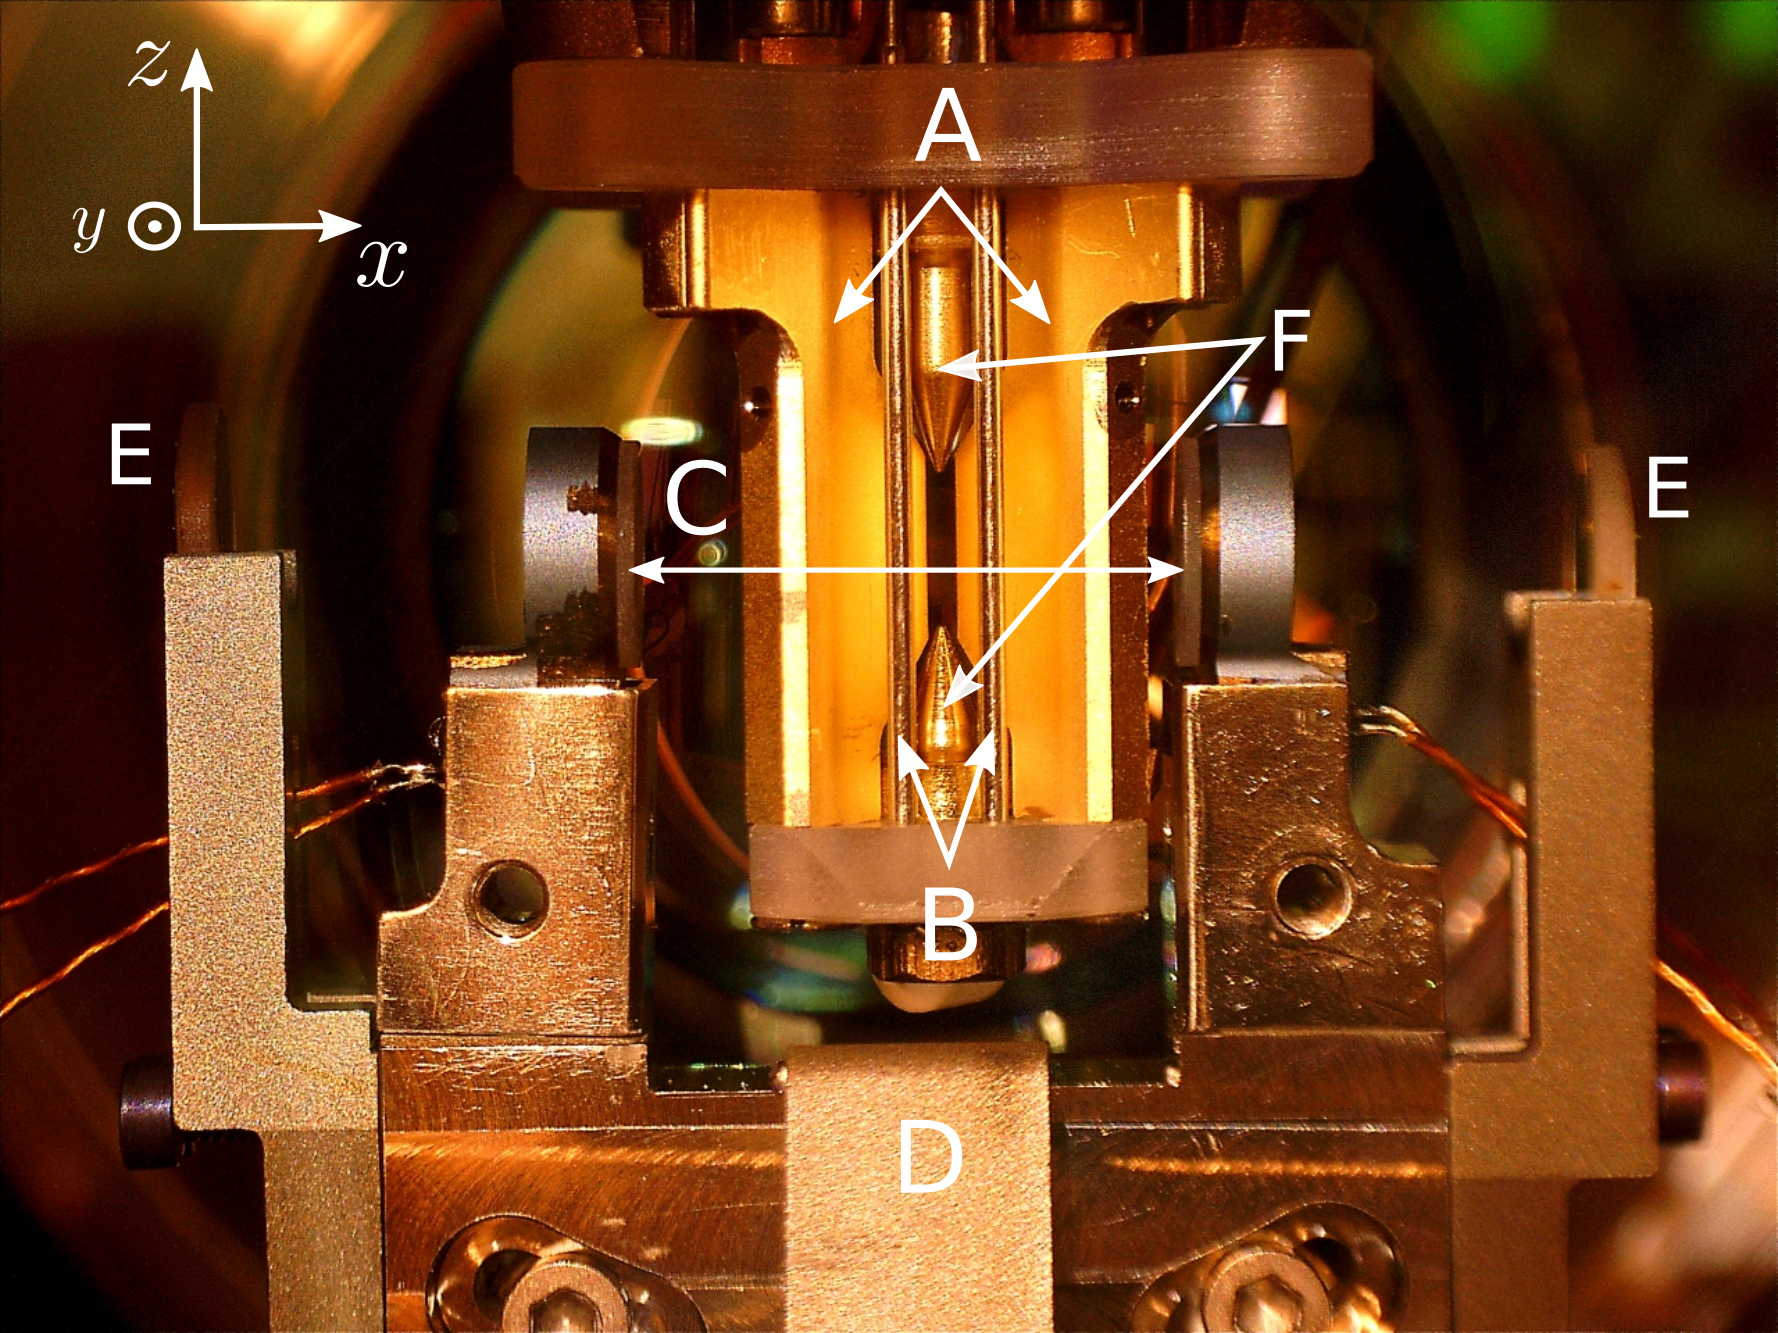
\includegraphics[width = .7\textwidth]{phototrap_white}
\caption{Photo of the mounted trap. The axial direction is defined along the $z$ axis, while radial is $r^2 = x^2 + y^2$. Highlighted in the image there are: (A) Trap's golden blades for radial RF confinement (B) One pair of compensation electrodes (C) Cavity mirrors, The left mirror is highly reflective, the right mirror is the 854 nm photon output mirror (see Section \ref{sec:cavityqed}), separation is $\sim 20$ mm (D) Calcium atomic oven (E) Collimation lenses (F) Static voltage endcaps for axial confinement.}
\label{trapphoto}
\end{figure}
In this section we discuss how to implement important techniques for ion based quantum computing and we present further key parameters of our experiment.\vspace{.5em}\\
\textbf{\textsc{Trapping and loading}}\\
Our trap is a linear 3D RF Paul trap as depicted in Figure \ref{trapphoto} where main components are highlighted. The electrodes are made of titanium and are coated in gold. The trap itself is mounted vertically on a shappire holder. The endcaps are 5 mm apart and are usually kept at voltages on the order of 500-1000V, which results in single-ion axial frequencies of $\omega_z \sim 2\pi \times 0.7-1$ MHz respectively. The four blades are 0.08 mm from the center of the trap and driven with an RF of $\sim 24$ MHz. The RF signal from an amplifier is impedance matched with the trap using a quarter-wave bulk helical resonator (not shown). The trap also includes three pairs of electrodes that can be used to compensate for stray electric fields. The location of the compensation electrodes, with respect to the trap, is presented later in Figure \ref{lossesplot}.\par
Loading of ions is done with a resistively-heated oven: calcium is heated and directed towards the trap, where neutral atoms undergo 2-stage photon ionization. First, a 422 nm laser resonantly excites one electron to the 4p$^1\text{P}_1$ state, while a second 375 nm laser, brings the electron to free space, ionizing the atom \cite{Gulde2001}. This two stage process allows for isotope selection ionizing only $^{40}\text{Ca}$. Loading usually takes minutes or tens of minutes depending on the number of ions one wants to load. Storage time can be in the order of days, especially when a single ion is loaded.\vspace{.5em}\\
\textbf{\textsc{Doppler cooling and Fluorescence imaging}}\\
Once loaded, ions are laser-cooled to the Doppler limit with 397 nm light on the transition $\text{S}_{1/2} \leftrightarrow \text{P}_{1/2}$ (Section \ref{sec:doppler_cooling}). An additional 866 nm repumper on the transition $\text{P}_{1/2} \leftrightarrow \text{D}_{3/2}$ is used to avoid the electron being stuck in the $\text{D}_{3/2}$ state. For typical experiments a stage of Doppler cooling is always included, typically lasting for a few milliseconds.\par
With the same lasers used for Doppler cooling, ion imaging and state readout are also done. The light shines on the ions exciting the transition $\text{S}_{1/2} \leftrightarrow \text{P}_{1/2}$ driving the electron to the excited state, which then decays spontaneously emitting photons. A fraction of the scattered 397 nm photons is collected with a custom objective with NA of $\sim 0.289$, which means a maximum possible efficiency of 2.5 \% of the solid angle $4\pi$. The objective focuses the collected photons 1.5 meters away where a CCD camera (Andor iXon Ultra 897) is placed. The geometrical path of the imaging photons is displayed in Figure \ref{imgsetup}, this setup has a magnification factor of $\sim$18.6. The same objective is also used for the addressing setup built within this thesis. Therefore, the imaging optical path must be partially shared with the newly built addressing. More details of the objective are given in Section \ref{sec:obj}.\vspace{.5em}\\
\textbf{\textsc{State readout with camera}}\\
Consider a qubit encoded in the states $\text{S}_{1/2}$ and $\text{D}_{5/2}$, if the imaging laser is switched on, the electron will be projected either to the $\text{S}_{1/2}$ level or to the $\text{D}_{5/2} $. In the first case, photons are scattered from the ion and collected on the camera, in the second case the electron is shelved and will not scatter any photon. Hence, the two cases are distinguishable by the brightness of the ion image on the camera. The camera can spatially separate the ions and therefore distinguish the individual state of each ion in the string. In order to perform this task, the camera software\footnote{Home developed software that works together with TrICS, see Section \ref{sec:expcontrol}} needs initial calibration. This means that a region of interest, where the fluorescing ions are, is first manually selected. The program takes the image in that region, integrates spatially in one direction (perpendicular to the string) and fits a number of Gaussians equal to the number of ions, where the central value of each peak indicates the position of each ions. The software then determines the brightness in one standard deviation interval and compares it with a previously set threshold determining ultimately the ion state. We thank Daniel Heinrich for developing this software.

\begin{figure}
\centering
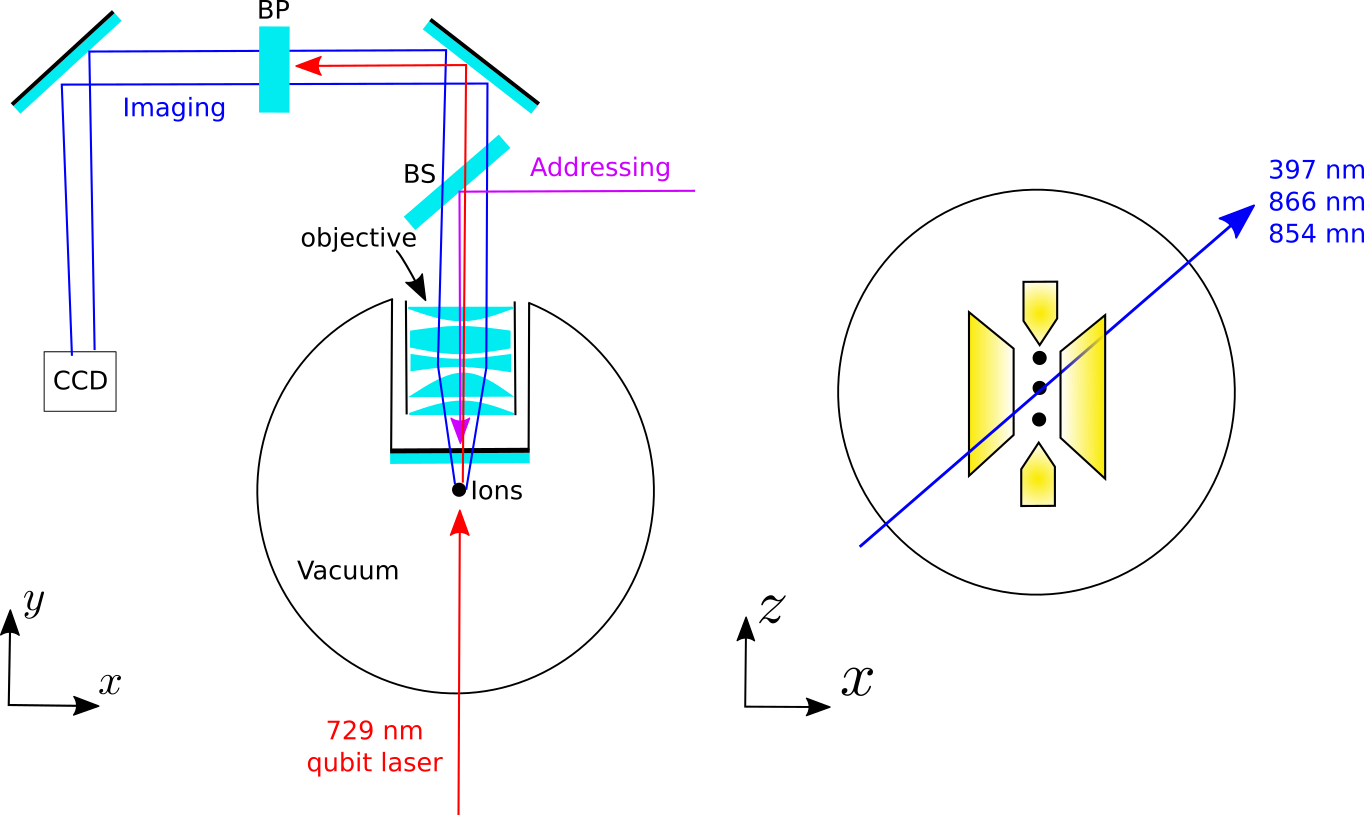
\includegraphics[width = .8\textwidth]{imgsetup}
\caption[Caption for LOF]{Left: top view of our ion trap system, an out-of-vacuum objective collimates and focuses the scattered 397 nm photons for imaging onto the CCD camera $\sim 1.5$ m away from the ions. The addressing setup must share part of this path, as the same objective is used for focusing the 393 nm laser.
A beam splitter (BS), installed during the course of this thesis, separates the imaging path from the addressing path. More details about the addressing path are in Section \ref{sec:addressing}.
A bandpass filter (BP) blocks the 729 nm light such that only 393 nm light can reach the camera. Right: front view of the trap, other laser directions are depicted.}
\label{imgsetup}
\end{figure}

\section{393 nm laser}
\label{sec:393setup}
\begin{figure}[!ht]
\centering
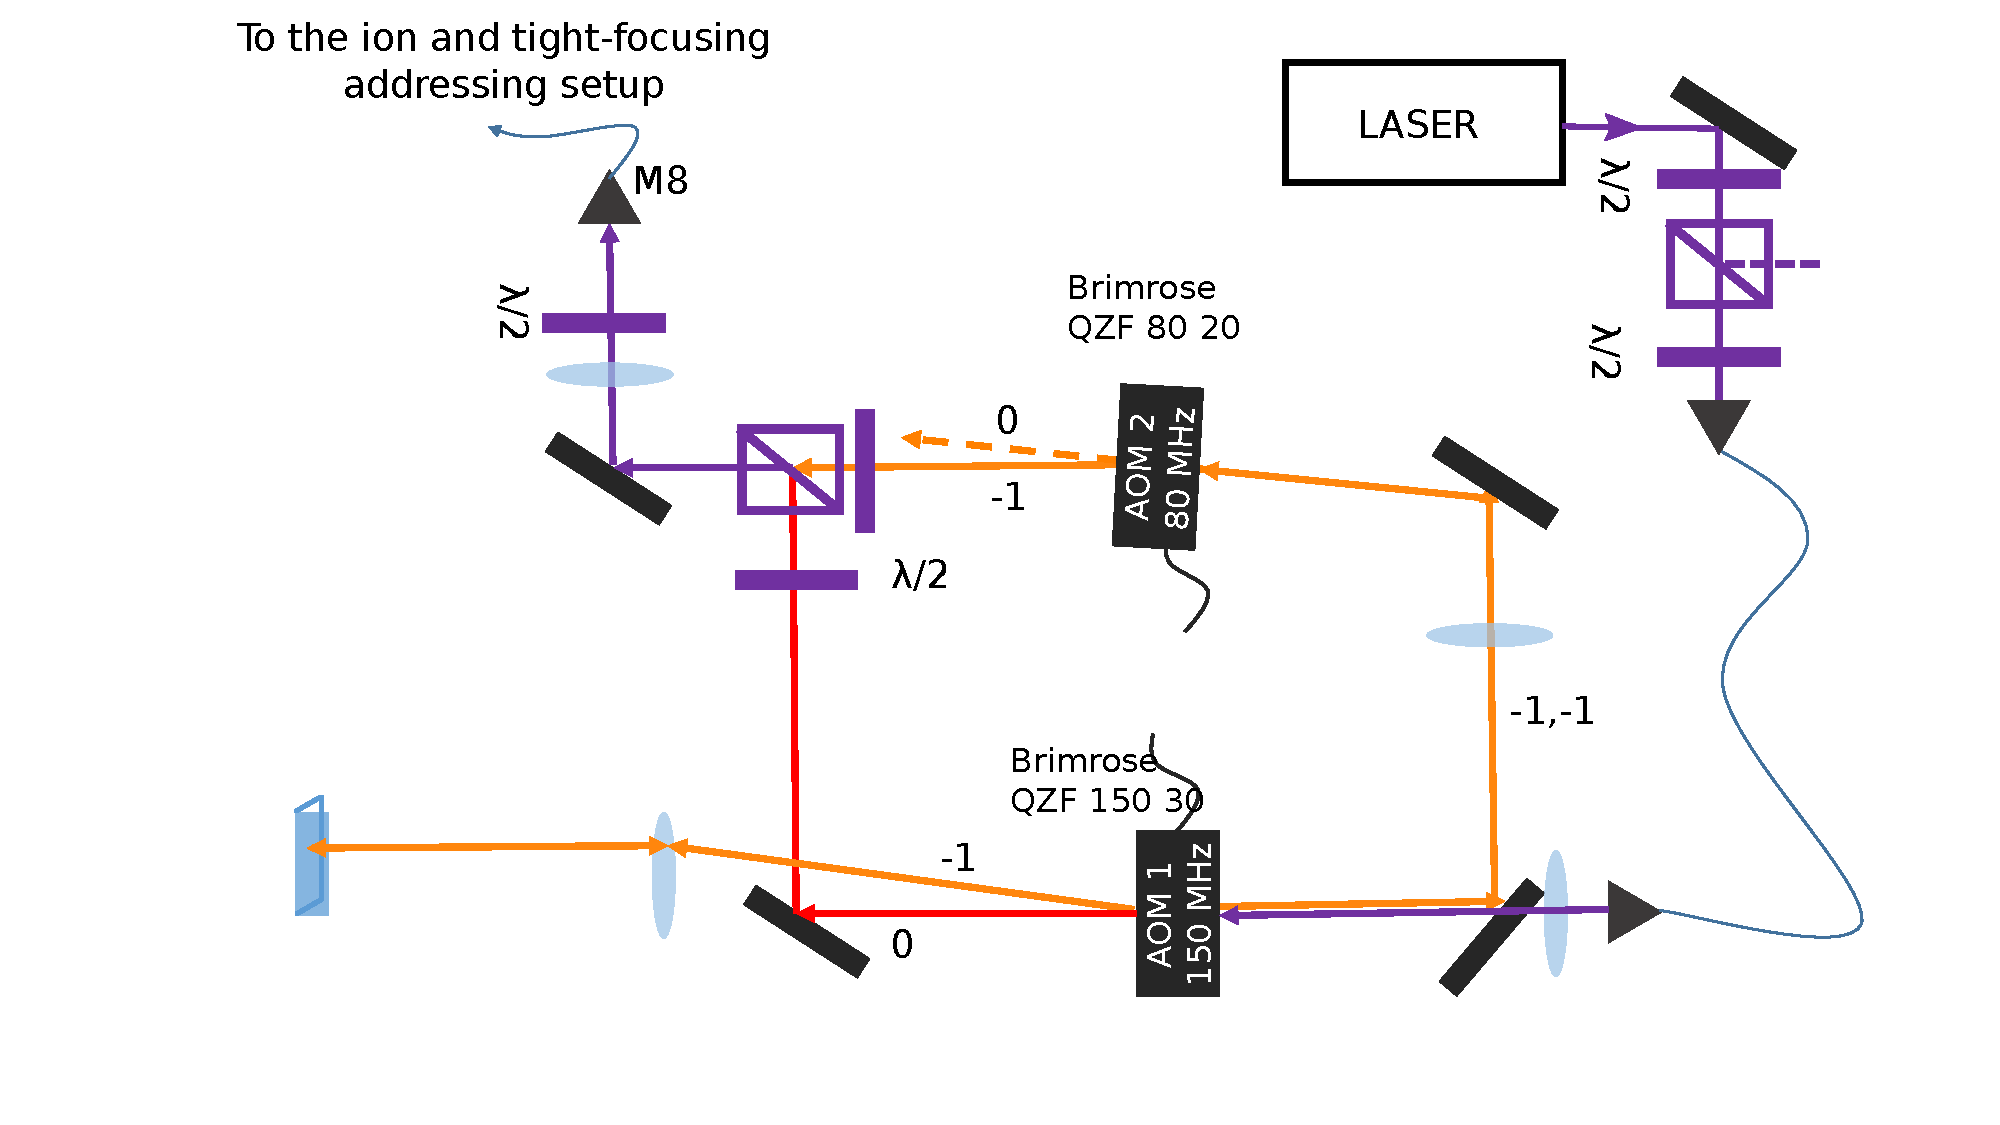
\includegraphics[width = \textwidth]{scheme_393}
\caption{393 nm laser optical setup before installation of the addressing system (a slight modification was required, see text). Two paths are present: a resonant path on the $\text{S}_{1/2} \leftrightarrow \text{P}_{3/2}$ transition (in red), and a detuned path (in orange) where a double pass AOM introduces -300 MHz shift, and a single pass AOM an additional -80 MHz. Paths are overlapped on a beam splitter and coupled to a fiber. A shutter can be used to block the resonant path. Numbers on the paths indicate diffraction order, above each AOM the model, central frequencies and bandwidths are shown, respectively. Setup built by V. Krutianskii, image made by him and adapted for this thesis.
}
\label{scheme393}
\end{figure}
The laser used to drive the addressed Raman transition is at 393 nm. This light is obtained from a titanium-sapphire laser from MSquared. The laser is optically pumped with 8 W of light at 532 nm from a Lighthouse Photonics Sprout laser. The Ti:Sa crystal is contained in a cavity in a bow tie configuration, together with an optical diode, etalon, birefringent mirror, and tunable cavity mirror for frequency tuning and stabilization. The laser can be frequency locked to a wavemeter or to an external cavity.\par
The fundamental light is set to 786 nm with tunability ranging from 725 nm to 875 nm that can be controlled remotely with a computer. The fundamental light is frequency doubled to 393 nm via an MSquared ECD-X external cavity resonant doubler accessory module. 393 nm light can be obtained with up to 1 W of power. Before reaching the ion trap, 393 nm light is sent through the setup in Figure \ref{scheme393}. The setup contains two paths: one resonant with the $\text{S}_{1/2} \leftrightarrow \text{P}_{3/2}$ transition, which goes directly to the ion; and a second path, where the light is detuned by -380 MHz for exciting the Raman transition described in Section \ref{sec:ramanprocess}.\par
The introduction of an AOD in the addressing setup shifts the light by -$125\pm25$ MHz. As we want to work around -400 MHz to excite the Raman transition, the setup in figure \ref{scheme393} had to be slightly altered to compensate for the additional AOD shift: AOM 2 was switched from -1 order to +1 order, and then driving frequencies were changed to 180 MHz for AOM 1 and 70 MHz for AOM 2.

\section{Experiment control}
\label{sec:expcontrol}
Our trapped-ion experiments require control over a large network of AOMs and other devices. Furthermore, precise control of the laser phase between sequential laser pulses, at the point of the ion, is also required, e.g. in the Ramsey experiments presented in this thesis. The need of fast and coherent pulse control is fulfilled by an electronic system that can be controlled with software on a central computer, from which every device connected to the network can be controlled. The experiment control network is sketched in Figure \ref{expcontrol}. The main components are:
\begin{itemize}
\item A computer: from here the experiment is controlled with TrICS (Trapped Ion Control Software)\footnote{A custom software developed internally in the Blatt  group of the University of Innsbruck used for controlling experiments based on trapped ions}.
\item Bus system\footnote{Designed in Innsbruck by G. Hendl.}: parallel communication system between the computer and various electronics such as Direct Digital Synthesizer (DDS).
\item Pulse box: FPGA and phase coherent DDSs that receive experiment sequences from the computer and generates accordingly coherent radio frequency pulses for key AOMs.
\end{itemize}
The computer is connected to the Bus system with a NIDAQ card. DDSs, used to generate radio frequency signal for AOMs, are connected to the Bus system through an optocoupler to avoid ground loops. The computer is connected via Ethernet and with another NIDAQ card to the Pulse Box. The card sends and receives trigger signals, while experiment sequences are uploaded to the Pulse box via the ethernet.\par
DDSs are used to generate RF signals that drive the AOMs, they set the frequency and the amplitude of the RF pulses. A set of TTL switches, controlled by the Pulse box, sets the length of the pulses generated by the DDSs connected to the Bus system. These DDSs are controlled on the $\mu$s timescale, switches instead are down to few nanoseconds timescale. DDSs in the pulse box are capable of a stable and controlled phase relationship and of switching the phase on the sub microsecond timescale. In the experiment of Section \ref{sec:singlequbitmanipulation}, Ramsey pulses need to be phase coherent, thus Pulse box DDSs had to be used. Moreover, during an experiment sequence, the parameters of the DDSs inside the pulse box can be varied, in contrast to DDSs on the Bus system whose frequency and amplitude have to be changed outside a sequence.\par
In a typical experiment, a sequence of pulses is programmed in Python on the computer. When the experiment is run, the computer uploads the sequence to the FPGA inside the Pulse Box. Next, the computer updates the DDSs on the Bus with the appropriate values for the experiment, sends a trigger signal to the Pulse Box and the Pulse Box generates and sends all the signals for the sequence. When the experiment is done, the Pulse box sends another trigger back to the computer, which proceeds to prepare for the next measurement point, it updates the values of the Bus DDSs, reuploads the code to the Pulse Box, sends a trigger to start the sequence and the loop is repeated.

\begin{figure}
\centering
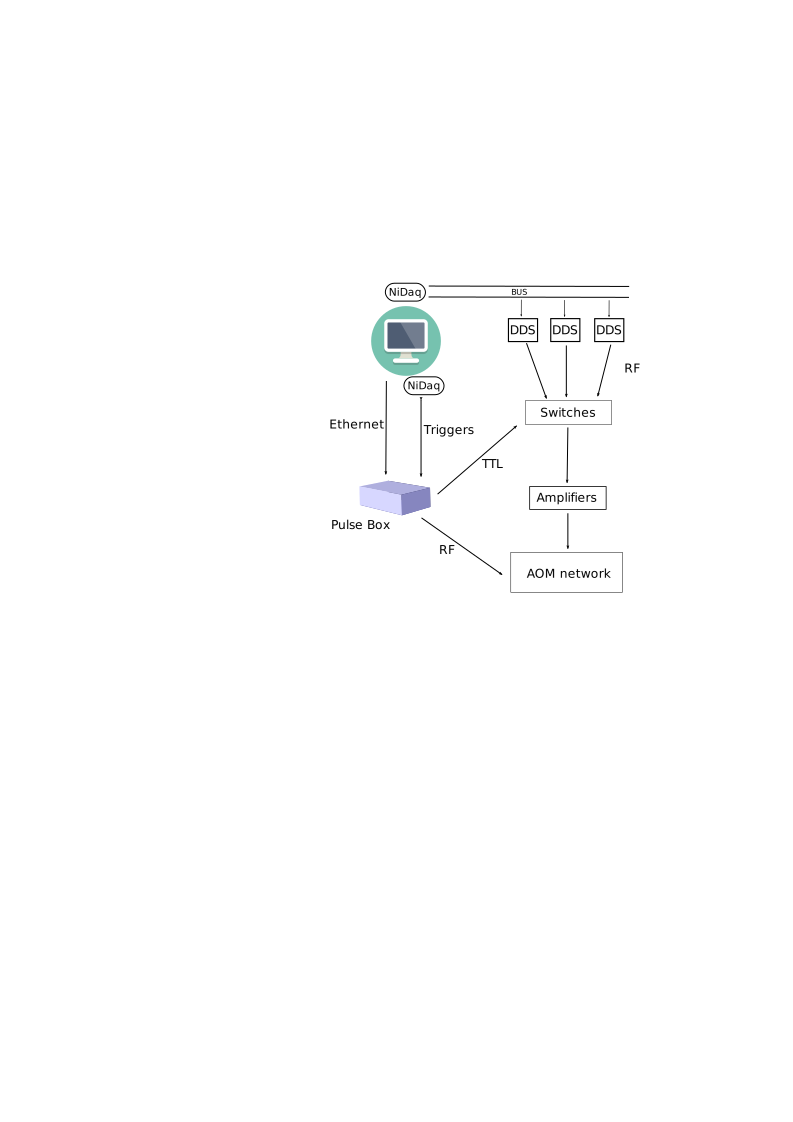
\includegraphics[width =.5\textwidth]{expcontrol}
\caption{Schematic of the experimental control. Everything is controlled remotely by a PC. During a sequence a pulse box generates coherent radio frequency pulses and digital voltages and sends them to various devices.}
\label{expcontrol}
\end{figure}

% \begin{figure}
% \centering
% 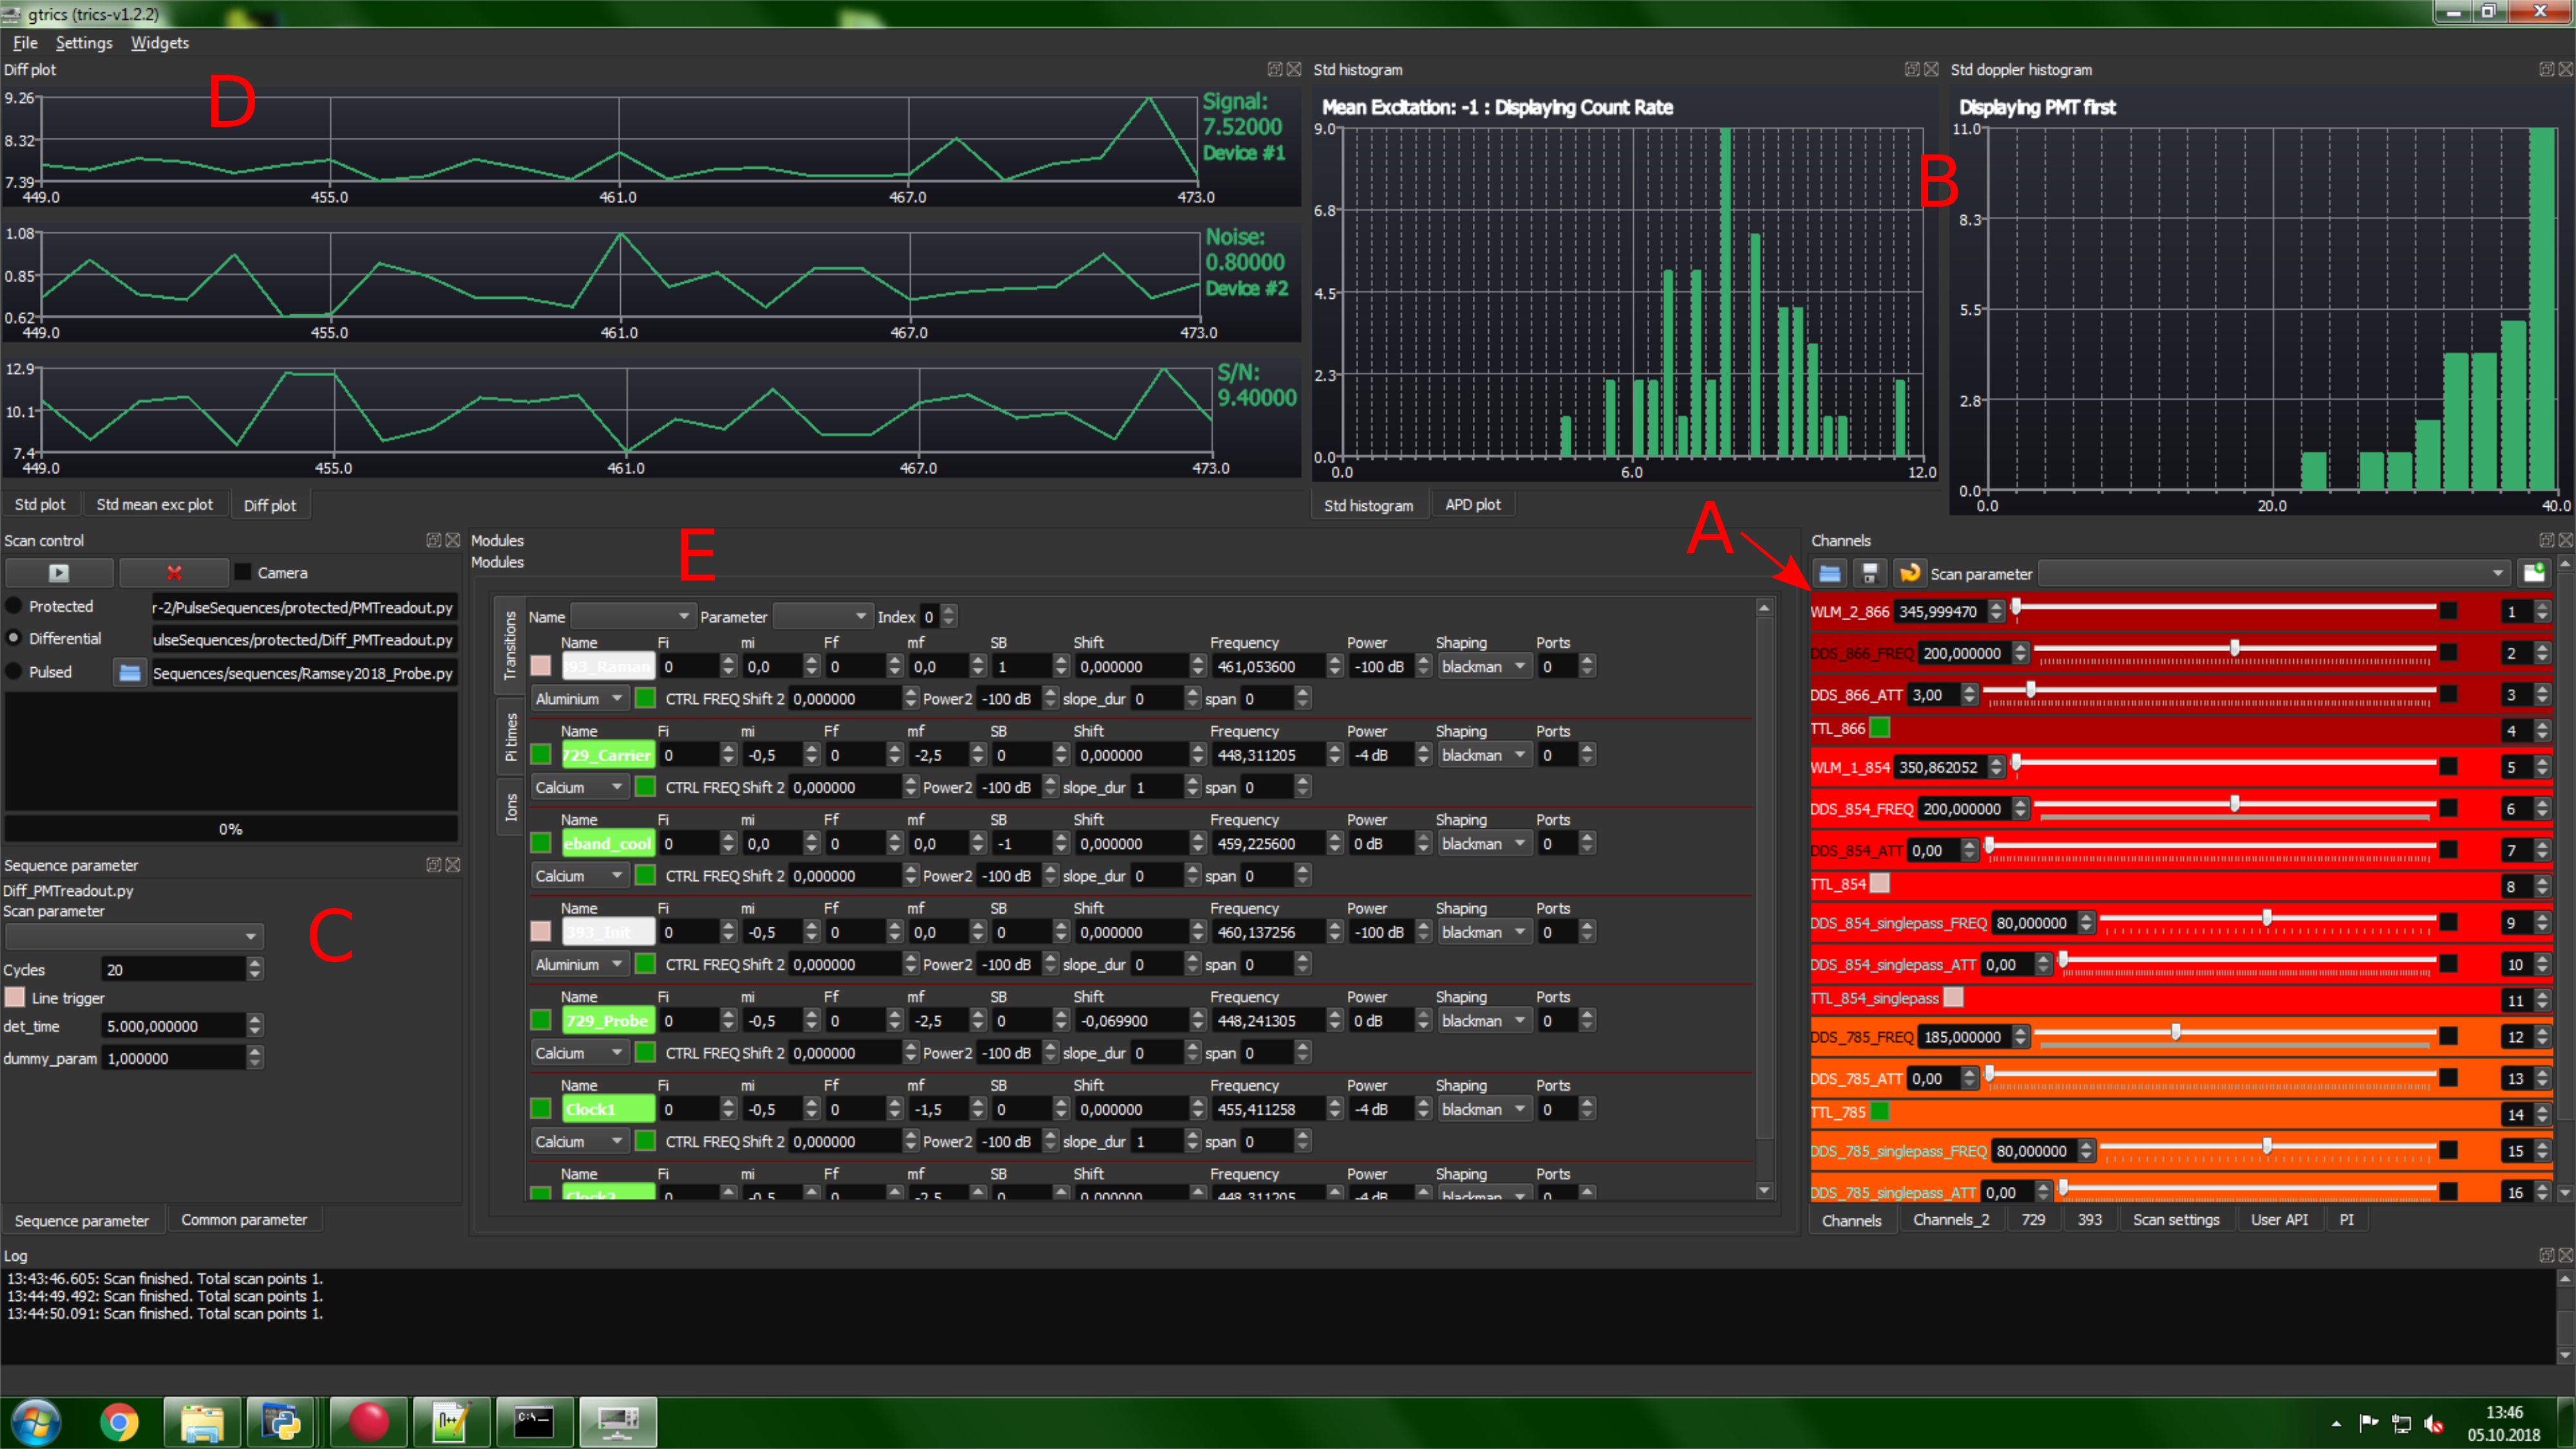
\includegraphics[width =\textwidth]{tricsmodified}
% \caption{Home developed TrICS software. We can see (A) Experimental device control, from here the user can add new devices and change their parameters, e.g. DDS frequency, switch ON/OFF, attenuation (B) photo multiplier tube (PMT) count histograms (C) Experiment scan control, from here experiment sequences can be launched (D) Various plots from PMT signal (E) Transition tab to store and modify information about ion transitions.}
% \label{trics}
% \end{figure}
